\newpage
\section{Kryptologie}
% TODO: 2 Teile im Pdf?
\section{Grundbegriffe und einfache Verfahren}
	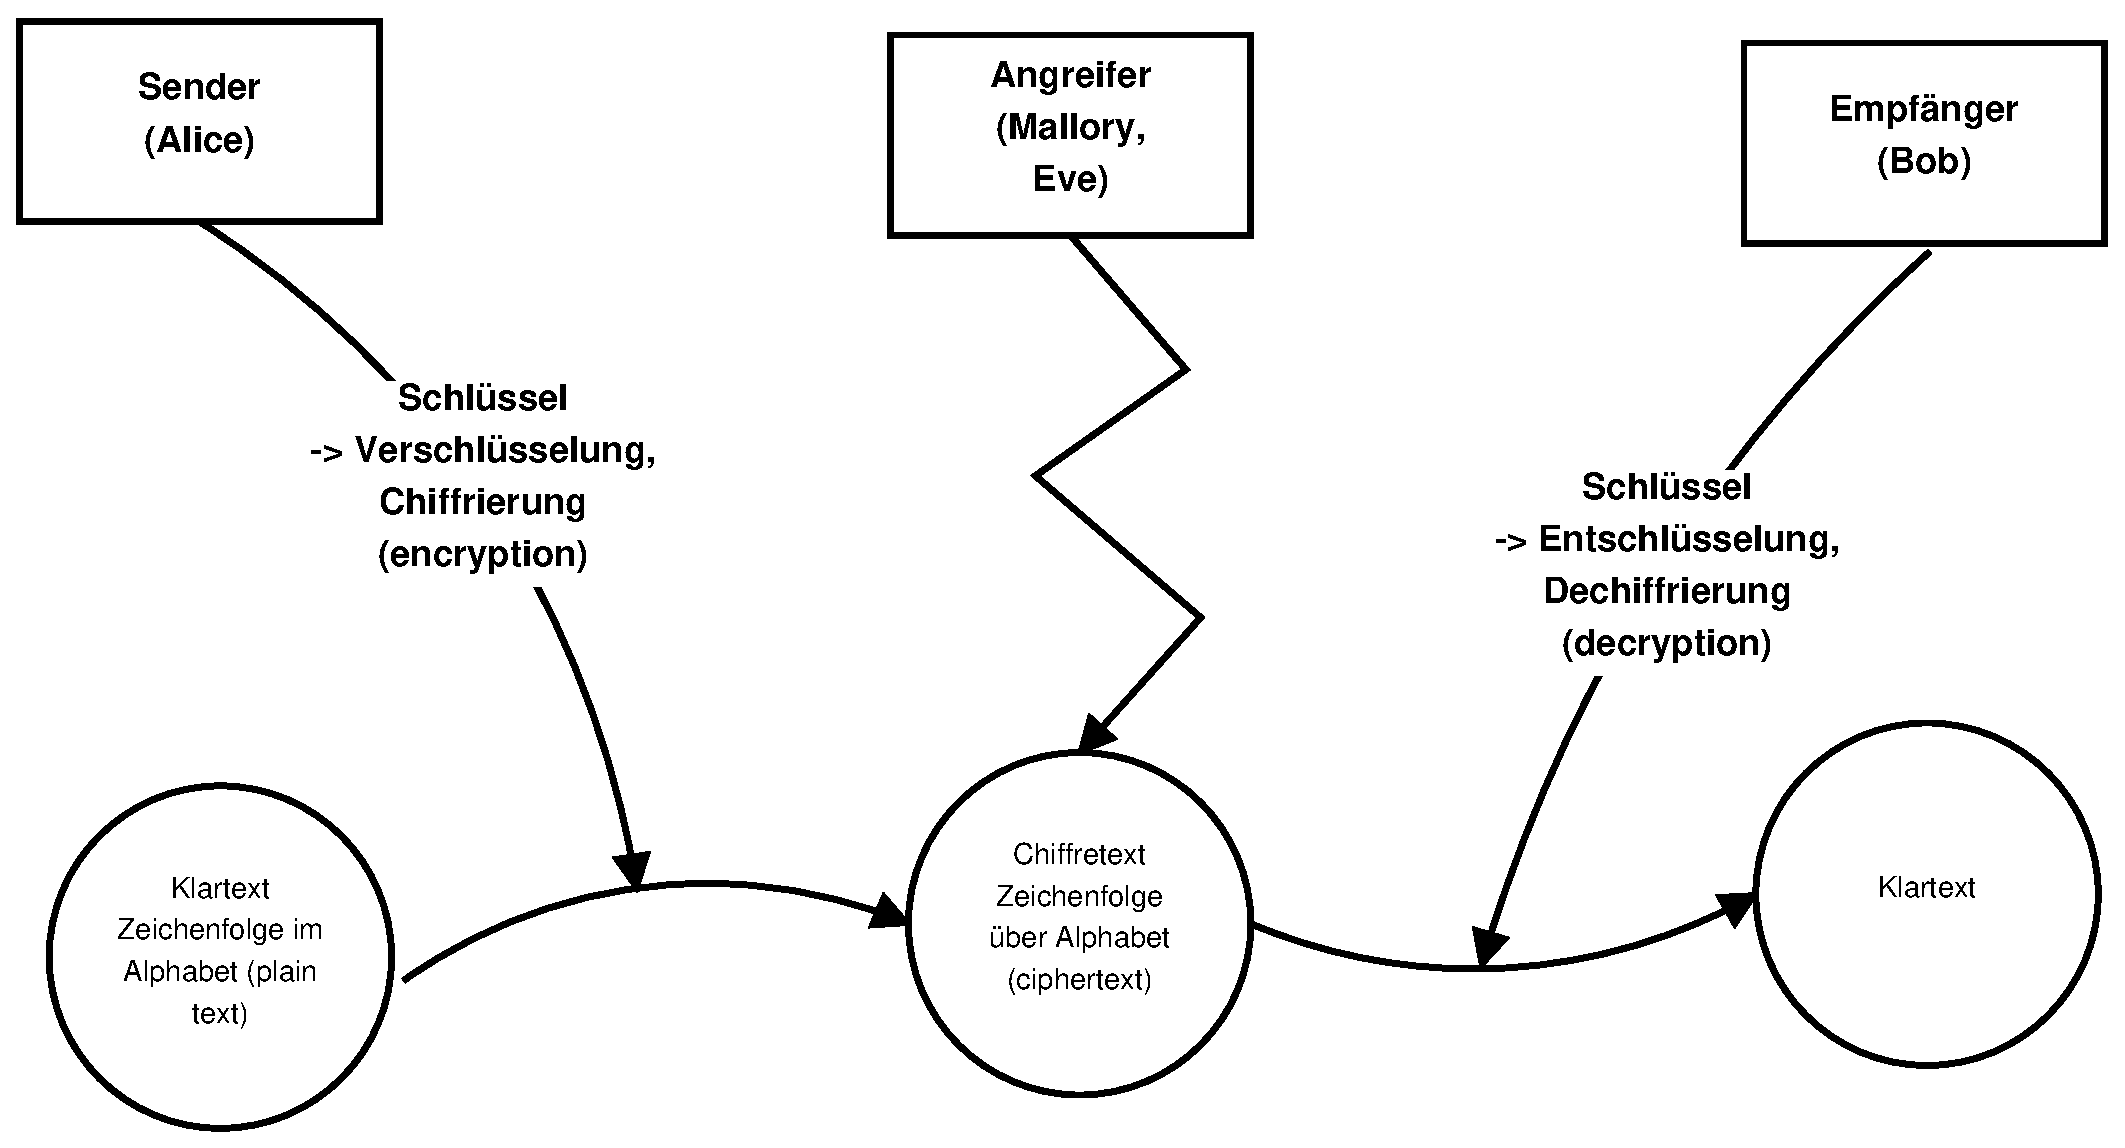
\includegraphics[width=\textwidth]{eps/pic01.eps}

	\textbf{Verschlüsselung erfordert}
	\begin{itemize}
		\item Verschlüsselungsverfahren, Chiffrieralgorithmus (Funktion $E$)
		\item Schlüssel $k_e$ (encryption key)
	\end{itemize}
	$E(\underset{\mbox{\scriptsize Klartext}}{m},\underset{\mbox{\scriptsize Schlüssel}}{k_e})=\underset{\mbox{\scriptsize Chiffretext}}{C}$ \\
	$k_e$ stammt aus der Menge $\mathcal{K}$ von Schlüsseln.\\
	Für ein festes $k_e$ muss $E\lrr{.,k_e}$ injektiv sein, das heißt\\
	$m_1\neq m_2 \Rightarrow E\lrr{m_1,k_e}\neq E\lrr{m_2,k_e}$
	
	\textbf{Entschlüsselung erfordert}
	\begin{itemize}
		\item Entschlüsselungsalgorithmus, Dechiffrierverfahren (Funktion $D$)
		\item Einen von $k_e$ abhängigen Decryption-Key $k_d$
	\end{itemize}
	$D(c,k_d)=m\quad D\lrr{.,k_d}=E\lrr{.,k_e}^{-1}$
	\subsection{Symmetrisches \& Asymmetrisches Verschlüsselungsverfahren}
		Ist $k_d=k_e$, oder falls $k_d$ leicht aus $k_e$ berechenbar ist, so spricht man von einem \textbf{symmetrischen Verschlüsselungsverfahren}.\\
		Lässt sich $k_d$ aus $k_e$ nur mit unverhältnismäßig großem Aufwand berechnen, so kann man $k_e$ öffentlich machen. Das heißt \textbf{Public Key Verfahren} oder auch \textbf{asymmetrisches VerschlÜsselungsverfahren}. (Kein Schlüsselaustausch notwendig!)
	
		In einem symmetrischen Verfahren werden $\binom{n}{2}=\dfrac{n\lrr{n-1}}{2}$ Schlüssel benötigt, wenn $n$ die Anzahl aller Verbindungspaare ist. Bei einem assymmetrischen Verfahren werden lediglich $2n$ Schlüssel benötigt.
	\subsection{Beispiel}
		\subExBegin{a)}
			\item $R=S=\lrc{0,\dots,25}$ \\
				Verfahren - \textbf{Verschiebechiffre}\\
				$\mathcal{K}=\lrc{0,\dots,25}$ \\
				Wähle Schlüssel $i\in\mathcal{K}$\\
				$x\in R$ Verschlüssle $x\rightarrow x+i\mod 26$\\
				$m=x_1\dots x_r\quad x_i\in R$\\
				$E\lrr{m,i}=\underbrace{\lrr{\lrr{x_1+i}\mod 26}}_{y_1}\dots\underbrace{\lrr{\lrr{x_r+i}\mod 26}}_{y_r}=c$\\
				Entschlüssle $y\in R \rightarrow y-i\mod 26$\\
				$D\lrr{c,i}=\lrr{\lrr{y_1-i}\mod 26}\dots\lrr{\lrr{y_r-i}\mod 26}=m$
			\item Verallgemeinerung: \textbf{Zeichenweise Substitutionschiffren}\\
				$R=S=\lrc{0,\dots,25} \quad\mathcal{K}=$ Menge der Permutationen von $R$\\
				Wähle $\pi\in\mathcal{K}$\\
				$m=x_1\dots x_r\quad x_i\in R$\\
				$E\lrr{m,\pi}=\underbrace{\pi\lrr{x_i}}_{y_1}\dots\underbrace{\pi\lrr{x_r}}_{y_r}=c$\\
				$c=y_1\dots y_r$\\
				$D\lrr{c,\pi^{-1}}=\pi^{-1}\lrr{y_1}\dots\pi^{-1}\lrr{y_r}=m$\\
				Jetzt ist $\lrabs{\mathcal{K}}=26!\equiv 4\cdot10^{26}$
			
				Angenommen ein Angreifer kann $10^{12}$ Schlüssel in der Sekunde testen.\\
				Angenommen $50\%$ der Schlüssel getestet werden um den richtigen zu finden.\\
				Dann werden $2\cdot 10^{14}$ Sekunden, also ungefähr $6.000.000$ Jahre benötigt.
		\subExEnd
	\subsection{Bemerkung}
		Das Verfahren aus 1.3b) ist bei Verschlüsselung von natürlichsprachlichen Texten völlig unsicher. Das liegt an der charakteristischen Buchstabenhäufigkeitsverteilung.
	\subsection{Prinzip von Kerkhoffs (1835-1903)}
		Die Sicherheit einer Verschlüsselung darf nicht von der Geheimhaltung des Verfahrens abhängen, sondern nur von der Geheimhaltung des Entschlüsselungsschlüssels $k_d$.
	\subsection{Kryptoanalyse}
		\begin{itemize}
			\item Ciphertext-Only-Angriff
			\item Known-Plaintext-Angriff
			\item Chosen-Plaintext-Angriff
			\item Chosen-Ciphertext-Angriff
	\end{itemize}
\section{One-Time-Pad und perfekte Sicherheit}
	\subsection{Lauftextverschlüsselungen}
		Klartext(über $R=\lrc{0,\dots,25}$) Wähle \textit{Schlüsseltext} der gleichen Länge über $R$\\
		Addiere Schlüsseltext zeichenweise zu Klartext $\mod 26$,
		
		\textbf{Beispiel}
		
		\begin{tabular}{lcccccccccc}
			Klartext&P&E&T&E&R&15&4&19&4&17\\
			Schlüsseltext&H&A&U&C&K&7&0&20&2&10\\\cline{7-11}
			&&&&&&22&4&13&6&1\\
			&&&&&&W&E&N&G&B
		\end{tabular}
		
		Das nennt sich \textbf{kontextabhängiges Verschlüsselungsverfahren}.
	\subsection{One-Time-Pad}
		Klartextalphabet $R=\lrc{0,1}=\mz_2$\\
		Klartext $m$ hat die Länge $n$ über $\mz_2$\\
		Wähle als Schlüsselfolge eine Zufallsfolge $k$ der Länge $n$ und addiere bitweise $\mod 2$ (XOR).\\
		$c=m\oplus k$
		
		\textbf{One-Time-Pad}: Schlüssel nur einmal verwenden.\\
		$c_1=m_1\oplus k$\\
		$c_2=m_2\oplus k$\\
		Angreifer fängt $c_1$ und $c_2$ ab:\\
		$c_1\oplus c_2 = m_1\oplus k\oplus m_2\oplus k=m_1\oplus m_2$\\
		Wenn $m_1,m_2$ sinnvolle Texte sind, so gibt es in $m_1\oplus m_2$ statistische Auffälligkeiten $\Rightarrow$ Angriffsmöglichkeiten.
		
		\begin{tabular}{lcccc}
		Klartext&$m_1$&$m_2$&\dots &$m_n$\\
		Schlüsselfolge&$S_1$&$S_2$&\dots &$S_n$\\
		$m_1\oplus S_1$&$m_2\oplus S_2$&\dots &$m_n\oplus S_n$
		\end{tabular}
		
	\subsection{Zufallsfolge der Länge \texorpdfstring{$n$}{n}}
		Erzeugt durch binäre symmetrische Quelle mit Wahrscheinlichkeit $50\%$ 0 oder 1, unabhängig von den schon erzeugten Bits. Also hat jede binäre Folge die Auftrittswahrscheinlichkeit $\dfrac{1}{2^n}$.
		
	\subsection{One- Time Pad ist unter den Voraussetzungen von 2.3/2.2 perfekt sicher}
		Das heißt für jeden Klartext $m$ und jeden denkbaren Chiffretext $c$ gilt:
		\[pr(m|c)=pr(m)\]
		$pr(m|c)$: a- priori Wahrscheinlichkeit für $m$, falls $c$ empfangen wurde.\\
		$pr(m)$: a- priori Wahrscheinlichkeit für $m$
		
		Warum ist One- Time- pad perfekt sicher?\\
		Formaler Beweis: Bayer'sche Formel\\
		Intuitiv: $m$ fester Klartext. $m\in\mz_2^n$\\
		Jeder Schlüssel $k\in\mz_2^n$ ist gleicher.\\
		$m\oplus k$ sind gleich wahrscheinlich, wenn $k$ über alle möglichen Schlüssel läuft.

\section{Symmetrische Blockchiffren}
	Blockchiffren $\underset{\mbox{\scriptsize Blöcke der Länge }n>1}{|\underbrace{\dots}|\underbrace{\dots}|\underbrace{\dots}|}$\quad Klartext
	
	Jeder Block wird einzeln verschlüsselt. Gleiche Blöcke werden gleich verschlüsselt (Es gibt aber auch andere Betriebsverschlüsselungen.\\
	$R=S=\mz_2$. Wie viele Blockchiffren der Länge $n$ gibt es?\\
	$\fbox{0...0}\fbox{0...01}\dots\dots\dots\fbox{1...1}$ $2^n$ Blöcke der Länge $n$\\
	Jeder dieser Blöcke wird in einen anderen umgewandelt\\
	Jeder Blockchiffre entspricht Permutation der $2^n$ Blöcke (Länge $n$) über $\mz_2$.\\
	Wenn alle Permutationen als Schlüssel zugelassen sind, so hat Schlüsselraum die Größe $\lrr{2^n}!$\\
Speicherbedarf für einen Schlüssel: $\underbrace{|*...*|*...*|\dots\dots\dots|*...*|}_{2^n\mbox{\scriptsize Blöcke mit }n\mbox{\scriptsize\ Bit}}$\\
	$n\cdot 2^n$ Bit, z.B. $n=64$\\
	Speicherung eines Schlüssels: $2^6\cdot 2^64=135\mbox{ TB}$
	
	\subsection{Lineare Blockchiffren}
		Klartextalphabet = Chiffretextalphabet = $\mz_k=\lrc{0,...,k-1}$\\
		Blocklänge $n$: Block $\in\mz^n$\\
		Block $m=(V_1,...,V_n)$, $V_i\in\mz_k$\\
		Schlüssel: $n\times n$- Matrix $A$ mit Einträgen in $\mz_k$ (und zusätzlicher Bedingung)\\
		Verschlüsselung: $c=m\cdot A=(w_1,...,w_n)$\\
		$\mz_5,n=2:\ (3,4)\cdot\lrv{1&2\\3&4}=\lrv{0&2}$\\
		$a\oplus b=a+b\mod k$\\
		Jedes Chiffrezeichen hängt von allen Klartextzeichen innerhalb eines Blocks ab\\(\textbf{Diffusion}).\\
		Wann ist diese Abbldung $m\in\mz_k^n\mapsto m\cdot A\in\mz_k^n$ injektiv, d.h. eine Permutation auf $\mz_k^n$?\\
		Genau dann, wenn $A$ invertierbar ist, d.h. $A^{-1}\ n\times n$- Matrix über $\mz_k$ mit der Eigenschaft $A^{-1}\cdot A=A\cdot A^{-1}=E_n=\begin{pmatrix}1&\dots&0\\\vdots&1&\vdots\\0&\dots&1\end{pmatrix}$\\
		Entschlüsseln: $c\cdot A^{-1}=(mA)\cdot A^{-1}=m(A\cdot A^{-1})=m\cdot E_n=m$
		
		$A\ n\times n$- Matrix über $\mz_k$, $\det(A)\in\mz_k$\\
		$2\times 2$- Matrix $\det\lrv{a&b\\c&d}a\cdot d-b\cdot c$\\
		$\mz_5:\ A=\lrv{1&2\\3&4}\quad\det(A)=(1\cdot 4-2\cdot 3)\mod 5=3$.
		
		$A$ invertierbar $\Leftrightarrow$ $\det(A)$ invertierbar in $\mz_k$ bezüglich $\odot$ $\Leftrightarrow\ \ggT(\det(A),k)=1$.\\
		$A^{-1}=(\det(A))^{-1}\cdot B$, $B=(b_{ij}),\ b_{ij}=(-1)^{i+j}\det(A_{ij})$\\
		$A_{ji}$ entsteht aus $A$ durch Streichen der $j$- ten Zeile und $i$- ten Spalte.\\
		Speziell $n=2$: $A=\lrv{a&b\\c&d}$, $\det(A)=ad-bc$\\
		$A^{-1}=\det(A)^{-1}\lrv{d&-b\\-c&a}$
		
		\textbf{Bsp.:} $\mz_6$, $A=\lrv{0&1\\1&3}$, $\det(A)=-1\mod 6=5$ $\ggT(5,6)=1$\\
		$5^{-1}=5$, da $5\odot 5=1$\\
		$A^{-1}=5^{-1}\lrv{3&-1\\-1&0}=\lrv{3&1\\1&0}$ über $\mz_6$.
		
		$m=(1,3)$\\
		Verschlüsselung: $m\cdot A=(1,3)\lrv{0&1\\1&3}=(3,4)=c\mod 6$\\
		Entschlüsselung: $c\cdot A^{-1}=(3,4)\lrv{3&1\\1&0}=(1, 3)=m$\\
		Schlüssel: $A$\\
		$\mz_2$: $n^2$ Bit.\\
		$n=64$. Wie viele invertierbare Matritzen $(64\times 64)$ über $\mz_8$ gibt es?\\
		$(2^{64}-1)(2^{64}-2)\dots(2^{64}-2^{63})\approx 0,29\cdot 2^{4061}$\\
		(Groß, aber winzig im Vergleich zu $\lrr{2^{64}}!\approx 2^{10^{21}}$)